%% LyX 2.4.4 created this file.  For more info, see https://www.lyx.org/.
%% Do not edit unless you really know what you are doing.
\documentclass[english,t]{beamer}
\usepackage{mathptmx}
\usepackage[T1]{fontenc}
\usepackage[latin9]{inputenc}
\usepackage{amssymb}
\usepackage{cancel}

\makeatletter
%%%%%%%%%%%%%%%%%%%%%%%%%%%%%% Textclass specific LaTeX commands.
% this default might be overridden by plain title style
\newcommand\makebeamertitle{\frame{\maketitle}}%
% (ERT) argument for the TOC
\AtBeginDocument{%
  \let\origtableofcontents=\tableofcontents
  \def\tableofcontents{\@ifnextchar[{\origtableofcontents}{\gobbletableofcontents}}
  \def\gobbletableofcontents#1{\origtableofcontents}
}

%%%%%%%%%%%%%%%%%%%%%%%%%%%%%% User specified LaTeX commands.
\usetheme{Warsaw}
% or ...

\setbeamercovered{transparent}
% or whatever (possibly just delete it)
\setbeamercovered{invisible} %makes overlays invisible

%gets rid of navigation symbols
\setbeamertemplate{navigation symbols}{}

%\usepackage{hyperref}
%\usepackage[usenames,dvipsnames,table]{xcolor} %adds additional color options
\definecolor{links}{HTML}{2A1B81}
%\hypersetup{colorlinks,linkcolor=blue,urlcolor=links}

\usepackage{multicol}

\usepackage{hyperref}

\usepackage{tikz}
\usetikzlibrary{calc}
\usetikzlibrary{plotmarks}
\usetikzlibrary{shapes}
\usepackage{pgfplots}
\pgfplotsset{compat=newest}

\usepackage{forest} %%for tree diagram

\usepackage{calc}
\usepackage[nomessages]{fp}

\usepackage[super]{nth} %easy 1st, 2nd, etc

%\usepackage{advdate}    % Advancing/saving dates
\usepackage{datetime}   % Dates formatting
%\usepackage{datenumber} % Counters for dates

\usepackage[super]{nth}

\usepackage{etex}

\usepackage{fancybox}

%%table colors
%\usepackage[table]{xcolor}
\usepackage{colortbl}

\usepackage[outline]{contour}  %allows text halos

\usepackage{epsdice} %%dice font
\usepackage[misc]{ifsym}
\newfont\dice{dice3d} %%3d dice font

\contourlength{1pt} %sets halo width
%%example: \node at (0.75,0.5) {\contour{white}{\Large Text!}};
%%example:  \node [fill=white,inner sep=1pt] at (2.25,0.5) {\Large 			Text!};
%%example:  \node [fill=white,rounded corners=2pt,inner sep=1pt] at 			(3.75,0.5) {\Large Text!};

%%%%%%%%%%%%%%%%%%%%%%%%%%%
\def\formatdateny{\csname noyear\languagename\expandafter\endcsname\formatdate}
\def\noyearenglish#1, \the\@year{#1}
\let\noyearamerican\noyearenglish
\let\noyearbritish\noyearenglish

%%allows uncover with forest diagrams
\tikzset{
    invisible/.style={opacity=0,text opacity=0},
    visible on/.style={alt=#1{}{invisible}},
    alt/.code args={<#1>#2#3}{%
      \alt<#1>{\pgfkeysalso{#2}}{\pgfkeysalso{#3}} % \pgfkeysalso doesn't change the path
    },
}
\forestset{
  visible on/.style={
    for tree={
      /tikz/visible on={#1},
      edge={/tikz/visible on={#1}}}}}

%%%redefines column alignment to match vertically
%\define@key{beamerframe}{t}[true]{% top
  %\beamer@frametopskip=.2cm plus .5\paperheight\relax%
  %\beamer@framebottomskip=0pt plus 1fill\relax%
 % \beamer@frametopskipautobreak=\beamer@frametopskip\relax%
  %\beamer@framebottomskipautobreak=\beamer@framebottomskip\relax%
  %\def\beamer@initfirstlineunskip{}%
%}

%%provides pdf with 4 slides per page; don't forget to add 'handout' to remove overlays
%\usepackage{pgfpages}
%\pgfpagesuselayout{4 on 1}[a4paper, landscape, border shrink=7mm]
%\pgfpageslogicalpageoptions{1}{border code=\pgfusepath{stroke}}
%\pgfpageslogicalpageoptions{2}{border code=\pgfusepath{stroke}}
%\pgfpageslogicalpageoptions{3}{border code=\pgfusepath{stroke}}
%\pgfpageslogicalpageoptions{4}{border code=\pgfusepath{stroke}}
%%%Don't forget to add 'handout'

\makeatother

\usepackage{babel}
\begin{document}
\newcommand{\xmax}{2000}
\newcommand{\xmin}{0}
\newcommand{\xstep}{0} %must be xmin+n
\newcommand{\ymax}{500}
\newcommand{\ymin}{0}
\newcommand{\ystep}{0} %must be ymin+n

\newcounter{countEx} \setcounter{countEx}{0}
\newcounter{countProb} \setcounter{countProb}{0}
\resetcounteronoverlays{countEx} \resetcounteronoverlays{countProb}

\newcommand{\ex}[3]{
	\addtocounter{countEx}{1}
	\only<#1-#2>{\begin{exampleblock} {Example \chNum.\secNum.\arabic{countEx}.} #3	\end{exampleblock}}
}

\newcommand{\prob}[4]{
	\addtocounter{countProb}{1}
	\only<#1-#2>{\begin{exampleblock} {Problem  \chNum.\secNum.\arabic{countProb}.\,#3} #4	\end{exampleblock}}
}

\newcommand{\yline}[4]{
	(#2 - #4)/(#1 - #3)*(x - #1) + #2
}

\beamerdefaultoverlayspecification{<+->}

%%%%Chapter and Section numbers%%%%%
\newcommand{\chNum}{3}
\newcommand{\secNum}{6}
\newcommand{\secTitle}{Mutually Exclusive and Independent Events}
\date{\formatdate{20}{10}{2014}}

\title[Section \chNum.\secNum: \secTitle]{Section \chNum.\secNum: \secTitle}

\subtitle{Finite Mathematics~~MTH 107~~Fall 2014}

\author{Dr.\,James Ashe}

\titlegraphic{\includegraphics[height=2.75cm]{/home/jim/JamesAshe/MHU/images/MarsHilUniversityLogo-Virtical.png}}

\institute{Mars Hill University}

\makebeamertitle 

%%True false command
\newcommand{\T}{\textcolor{green}{\contour{black}{T}}}
\newcommand{\F}{\textcolor{red}{\contour{black}{F}}}
\newcommand{\uT}[2]{\uncover<#1-#2>{\T}}
\newcommand{\uF}[2]{\uncover<#1-#2>{\F}}

%tkiz ball item 
\newcommand*\circled[1]{\tikz[baseline=(char.base)]
	{\node[circle,ball color=green!50!black!100, shade,   color=white,inner sep=1.2pt] (char) {\tiny #1};
	}
}
\begin{frame}{Independent/Dependent Events}

\vspace{-.5cm}
\begin{columns}


\column{5cm}
\begin{block}<1->{Independent}
Two events, $A$ and $B$, are \emph{independent }if $p(A\mid B)=p(A)$.
\end{block}
\begin{itemize}
\item []<2->\emph{Knowing B does not effect A's probability.}
\end{itemize}
\begin{block}<3->{dependent}
Two events, $A$ and $B$, are \emph{dependent }if $p(A\mid B)\neq p(A)$.
\end{block}
\begin{itemize}
\item []<4->\emph{Knowing B does effect A's probability.}
\end{itemize}

\column{6cm}

\ex{5}{6}{Two cards are dealt (without replacement). Are the events
independent?
\begin{itemize}
\item [J:] A jack is dealt \nth{1}
\item [H:] A queen is dealt \nth{2}
\item []<6->No. Dependent.
\end{itemize}
}

\ex{7}{8}{Two dice are rolled. Are the events independent?
\begin{itemize}
\item [4:]The \nth{1} die is $4$
\item [2:]The \nth{2} die is $2$
\item []<8->Yes. Independent.
\end{itemize}
}

\ex{9}{10}{Two dice are rolled. Are the events independent?
\begin{itemize}
\item [E:]The roll is even.
\item [2:]A $2$ is rolled.
\item []<10->No. Dependent.
\end{itemize}
}
\end{columns}
\end{frame}

\begin{frame}{The Product Rule}

\begin{columns}


\column{5cm}
\begin{block}<2->{Product Rule}
$p(A\cap B)=p(A\mid B)\cdot p(B)$
\end{block}

\begin{block}<11->{Product Rule for Independent Events}
$p(A\cap B)=p(A)\cdot p(B)$
\end{block}

\column{6cm}

\ex{3}{7}{Two cards are dealt (without replacement). Find $p(J\cap H)$.
\begin{itemize}
\item [J:] A jack is dealt \nth{1}
\item [H:] A queen is dealt \nth{2}
\end{itemize}
}

\only<4-7>{
\begin{itemize}
\item []$p(H\cap J)=p(H\mid J)\cdot p(J)$
\item []<5->\hspace{0cm}\hphantom{$p\cap J$}$=p(H\mid J)\cdot\dfrac{4}{52}$
\item []<6->\hspace{0cm}\hphantom{$p\cap J$}$=\dfrac{4}{51}\cdot\dfrac{4}{52}=\dfrac{16}{51\cdot52}$
\item []<7->\hspace{0cm}\hphantom{$p\cap J$}$\approx.0060$
\end{itemize}
}

\ex{8}{12}{A cards is dealt, replaced, and another card is dealt.
Find $p(J\cap H)$.
\begin{itemize}
\item [J:] A jack is dealt \nth{1}
\item [H:] A heart is dealt \nth{2}
\end{itemize}
}

\only<9-12>{
\begin{itemize}
\item []$p(H\cap J)=p(H\mid J)\cdot p(J)$
\item []<10->\hspace{0cm}\hphantom{$p\cap J$}$=p(H\mid J)\cdot\dfrac{4}{52}$
\item []<11->\hspace{0cm}\hphantom{$p\cap J$}$=\dfrac{4}{52}\cdot\dfrac{4}{52}=\dfrac{16}{52^{2}}$
\item []<12->\hspace{0cm}\hphantom{$p\cap J$}$\approx.0059$
\end{itemize}
}

\ex{13}{16}{Two dice are rolled. Find $p(4\cap2)$.
\begin{itemize}
\item [4:]The \nth{1} die is $4$
\item [2:]The \nth{2} die is $2$
\end{itemize}
}

\only<14-16>{
\begin{itemize}
\item []$p(4\cap2)=p(4\mid2)\cdot p(2)$
\item []<15->\hspace{0cm}\hphantom{$p\cap J$}$=p(4\mid2)\cdot\dfrac{1}{6}$
\item []<16->\hspace{0cm}\hphantom{$p\cap J$}$=\dfrac{1}{6}\cdot\dfrac{1}{6}=\dfrac{1}{36}$
\end{itemize}
}

\ex{17}{20}{Two dice are rolled. Find $p(2\cap E)$.
\begin{itemize}
\item [E:]The roll is even.
\item [2:]A $2$ is rolled.
\end{itemize}
}

\only<18-20>{
\begin{itemize}
\item []$p(2\cap E)=p(2\mid E)\cdot p(E)$
\item []<19->\hspace{0cm}\hphantom{$p\cap J$}$=p(2\mid E)\cdot\dfrac{18}{36}$
\item []<20->\hspace{0cm}\hphantom{$p\cap J$}$=\dfrac{1}{18}\cdot\dfrac{18}{36}=\dfrac{1}{36}$
\item []<21->note: $p(2)=\dfrac{1}{36}\neq\dfrac{1}{18}=p(2\mid E)$
\end{itemize}
}
\end{columns}
\end{frame}

\begin{frame}{Mutually Exclusive}

\vspace{-.5cm}
\begin{columns}


\column{5.5cm}
\begin{block}<1->{Recall:}
Two sets, $A$ and $B$, are \emph{mutually disjoint/exclusive }if
$A\cap B=\emptyset$
\end{block}

\begin{block}<1->{}
Two events, $A$ and $B$, are \emph{mutually exclusive }if $A\cap B=\emptyset$
\end{block}

\column{5.5cm}

\only<2->{%%%% M and A %%%%%
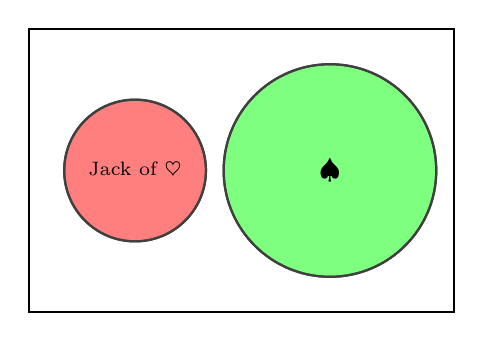
\begin{tikzpicture}[scale=.9]
	\def\circleA{(-.5,0) circle (1)} %A
	\def\circleB{(0:2.25) circle (1.5)} %B

	\colorlet{circle edgeA}{black!75} 
	\colorlet{circle areaA}{red!100}
	\colorlet{circle edgeB}{black!75} 
	\colorlet{circle areaB}{green!100}

	\tikzset{
		filledA/.style={fill=circle areaA, draw=circle edgeA, thick},
		filledB/.style={fill=circle areaB, draw=circle edgeB, thick},
		outlineA/.style={draw=circle edgeA, thick},
		outlineB/.style={draw=circle edgeB, thick},
	}
	
	\begin{scope}[fill opacity=0.5]         
			\fill[filledA] \circleA;
			\fill[filledB] \circleB;    
	\end{scope}

	\draw[outlineA] \circleA node[] {\scriptsize Jack of $\heartsuit$}; 
	\draw[outlineB] \circleB node[] {$\spadesuit$};
	\draw (1,0) node {};
	\draw[thick] (-2,-2) rectangle (4,2) node[anchor=south east] at (current bounding box.south east) {$$}; 
	%\node[anchor=south] at (current bounding box.north) {Prob Passes at least 1}; 
\end{tikzpicture} }

\vspace{-.5cm}
\end{columns}
\begin{itemize}
\item <4->Recall: \only<4-6>{If $A\cap B=\emptyset$ then $p(A\cup B)=p(A)+p(B)$}\only<9->{If
$A\cap B=\emptyset$ then $p(A\cap B)=0$}
\item <5->[ex.]The probability of drawing a $J\heartsuit$ OR a $\spadesuit$
is:

\begin{itemize}
\item <6->[]$p(J\heartsuit\cup\spadesuit)=\dfrac{1}{52}+\dfrac{13}{52}=\dfrac{14}{52}$
\end{itemize}
\item <7->[ex.]The probability of drawing a $J\heartsuit$ AND a $\spadesuit$
is:

\begin{itemize}
\item <8->[]$p(J\heartsuit\cap\spadesuit)=\dfrac{n(J\heartsuit\cap\spadesuit)}{n(S)}=\dfrac{0}{52}=0$
\end{itemize}
\end{itemize}
\end{frame}

\begin{frame}{Problems}

\prob{1}{1}{A group of doctors found the following about their patients}{
\begin{itemize}
\item They had 400 clients.
\item 250 have ankle problems.
\item Of patients with ankle problems, 200 only run.
\item Of patients without ankle problems, 25 only run.
\item [a.]Are the events ``running only'' and ``having ankle problems''
independent or dependent?
\item [b.]Are the events ``running only'' and ``having ankle problems''
mutually exclusive?
\item [c.]Does only running increase the probability of ankle problems?
\end{itemize}
}

\prob{2}{2}{A card is dealt from a full deck}{
\begin{itemize}
\item [a.]Find the probability of being deal a jack, $p(J)$.
\item [b.]Find the probability of being deal a jack given that you were
dealt a card above 10, $p(J\mid C>10)$.
\item [c.]Are the events ``$J$'' and ``$C>10$:'' independent?
\item [d.]Are the events ``$J$'' and ``$C>10$:'' mutually exclusive?
\item [e.]Does dependent$\rightarrow$mutually exclusive?
\end{itemize}
}
\end{frame}

\begin{frame}{Exam 3}

\begin{itemize}
\item []
\item Exam 3 is on \formatdate{27}{10}{2014}
\item The review session is from 7pm-9pm on \formatdate{26}{10}{2014} in
the RI classroom of the library.
\end{itemize}
\end{frame}

\end{document}
